% !TEX TS-program = xelatex
%
\documentclass[aspectratio=1610]{beamer}

\makeatletter
\@ifclassloaded{beamer}{
  \usetheme{metropolis}

  \usepackage{fontspec}
  \defaultfontfeatures{Ligatures=TeX}

  \usefonttheme{professionalfonts}
  \usepackage[familydefault,light]{Chivo}
}{
  \linespread{1.25}
}
\makeatother

\usepackage{graphicx}
\usepackage{graphbox}
\graphicspath{ {../assets/} }

\usepackage{hyperref}
\usepackage{cleveref}
\usepackage{nameref}

\usepackage[
  binary-units = true,
  per-mode     = symbol,
]{siunitx}

\usepackage[export]{adjustbox}
\usepackage{tabularx}

\usepackage{listings}

% http://latexcolor.com
\definecolor{gray}{rgb}{0.5, 0.5, 0.5}
\definecolor{ceruleanblue}{rgb}{0.16, 0.32, 0.75}
\definecolor{green(ncs)}{rgb}{0.0, 0.62, 0.42}
\definecolor{auburn}{rgb}{0.43, 0.21, 0.1}

% https://tex.stackexchange.com/a/83100
\colorlet{punct}{red!60!black}
\definecolor{delim}{RGB}{20,105,176}

\lstdefinelanguage{mongo}{
  basicstyle        = \normalfont\ttfamily,
  showstringspaces  = false,
  breaklines        = true,
  stringstyle       = \color{green(ncs)},
  morestring        = *[b]{'},
  morestring        = *[b]{"},
  morestring        = *[b]{`},
  literate          =
    *{:}{{{\color{punct}{:}}}}{1}
    {,}{{{\color{punct}{,}}}}{1}
    {\{}{{{\color{delim}{\{}}}}{1}
    {\}}{{{\color{delim}{\}}}}}{1}
    {[}{{{\color{delim}{[}}}}{1}
    {]}{{{\color{delim}{]}}}}{1},
}

% https://tex.stackexchange.com/a/152856
\newcommand\YAMLcolonstyle{\color{red}\mdseries}
\newcommand\YAMLkeystyle{\color{black}\bfseries}
\newcommand\YAMLvaluestyle{\color{auburn}\mdseries}

\lstdefinelanguage{yaml}{
  keywords      = {true,false,null,y,n},
  keywordstyle  = \color{gray},
  basicstyle    = \normalfont\ttfamily,
  sensitive     = false,
  comment       = [l]{\#},
  morecomment   = [s]{/*}{*/},
  commentstyle  = \color{purple},
  stringstyle   = \color{green(ncs)},
  moredelim     = [l][\color{orange}]{\&},
  moredelim     = [l][\color{magenta}]{*},
  moredelim     = **[il][\YAMLcolonstyle{:}\YAMLvaluestyle]{:},
  morestring    = [b]',
  morestring    = [b]",
}

% http://mirrors.ibiblio.org/CTAN/macros/latex/contrib/listings/lstdrvrs.pdf

\lstdefinelanguage{Ruby}{
  morekeywords       = {\_\_FILE\_\_,\_\_LINE\_\_,BEGIN,END,alias,and,begin,break,
  case,class,def,defined?,do,else,elsif,end,ensure,false,for,
  if,in,module,next,nil,not,or,redo,rescue,retry,return,self,
  super,then,true,undef,unless,until,when,while,yield,task,namespace,
  cd,sh,rm_rf,cp_r,desc,puts,mkdir_p,each},
  sensitive          = true,
  morecomment        = [l]\#,
  morecomment        = [l]\#\#,
  morecomment        = [s]{=BEGIN}{=END},
  morestring         = [b]',
  morestring         = [b]’,
  morestring         = [b]",
  morestring         = [s]{\%q/}{/},
  morestring         = [s]{\%q!}{!},
  morestring         = [s]{\%q\{}{\}},
  morestring         = [s]{\%q(}{)},
  morestring         = [s]{\%q[}{]},
  morestring         = [s]{\%q-}{-},
  morestring         = [s]{\%Q/}{/},
  morestring         = [s]{\%Q!}{!},
  morestring         = [s]{\%Q\{}{\}},
  morestring         = [s]{\%Q(}{)},
  morestring         = [s]{\%Q[}{]},
  morestring         = [s]{\%Q-}{-}
  breaklines         = true,
  basicstyle         = \normalfont\ttfamily,
  breaklines         = true,
  showstringspaces   = false,
  identifierstyle    = \color{auburn},
  commentstyle       = \color{gray},
  keywordstyle       = \color{ceruleanblue},
  stringstyle        = \color{green(ncs)},
  rangeprefix        = \#\#\#\ ,
  rangebeginsuffix   = \ begin,
  rangeendsuffix     = \ end,
  includerangemarker = false,
}[keywords,comments,strings]

\lstdefinelanguage{bash}{
  keywords           = {true,false,null,if,fi,esac,case,exec,echo},
  keywordstyle       = \color{auburn},
  basicstyle         = \normalfont\ttfamily,
  morestring         = [b]',
  morestring         = [b]’,
  morestring         = [b]",
  morecomment        = [l]\#,
  morecomment        = [l]\#\#,
  showstringspaces   = false,
  commentstyle       = \color{red},
  keywordstyle       = \color{ceruleanblue},
  stringstyle        = \color{green(ncs)},
}

\newcommand{\whitelist}[1]{#1}

\title{IoT Data Analytics \\ using Serverless Computing}
\author{Michael Kaltschmid \\ 01518956 \\ \hfill \\ Markus Reiter \\ 01518446}
\date{}


\newcolumntype{R}{>{\raggedleft\arraybackslash}X}
\newcolumntype{C}{>{\centering\arraybackslash}X}

\begin{document}
  \maketitle

  \begin{frame}{Outline}
    \begin{itemize}
      \item Introduction
      \item What is the Internet of things?
      \item What is serverless computing?
      \item Devices
      \item Background
      \item Implementation
      \item Results
      \item Schedule
    \end{itemize}
  \end{frame}

  \begin{frame}{Introduction}
    \begin{itemize}
      \item collect data from various devices
      \item devices post data to broker
      \item serverless function called depending on data type
      \item data saved in database
      \item web application to visualize data and statistics
    \end{itemize}
  \end{frame}

  \begin{frame}{What is the Internet of things (IoT)?}
    \begin{itemize}
      \item everyday objects (things) connected to the Internet
      \item collection of switches and sensors
      \item controlled or monitored remotely via the Internet or by other IoT devices
    \end{itemize}
  \end{frame}

  \begin{frame}{What is serverless computing?}
    \begin{itemize}
      \item confusing name, actually still requires servers
      \item cloud provider runs master server
      \item master server manages scaling and allocates resources
      \item functions deployed on-demand
    \end{itemize}
  \end{frame}

  \begin{frame}{Devices: Smartphone}
    \begin{itemize}
      \item gyroscope
            \hspace*{2em}
            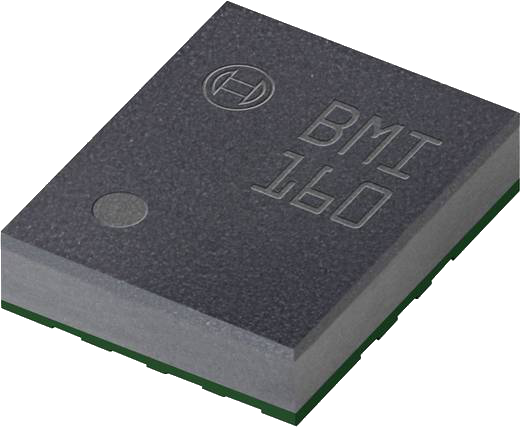
\includegraphics[align=c,height=3em]{bmi160-sensor}
      \item accelerometer
      \item magnetometer
      \item barometer
            \hspace*{2em}
            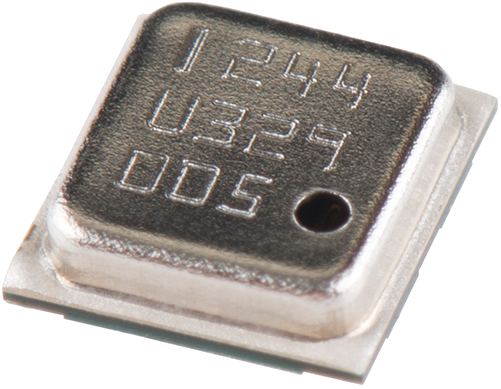
\includegraphics[align=c,height=3em]{barometric-sensor}
      \item gravity
      \item temperature
      \item humidity
            \hspace*{2em}
            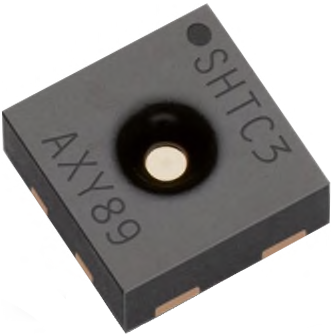
\includegraphics[align=c,height=3em]{shtc3-humidity-sensor}
      \item possibly GPS location
    \end{itemize}
  \end{frame}

  \begin{frame}{Devices: Raspberry Pi}
    \begin{itemize}
      \item temperature sensor
            \hspace*{2em}
            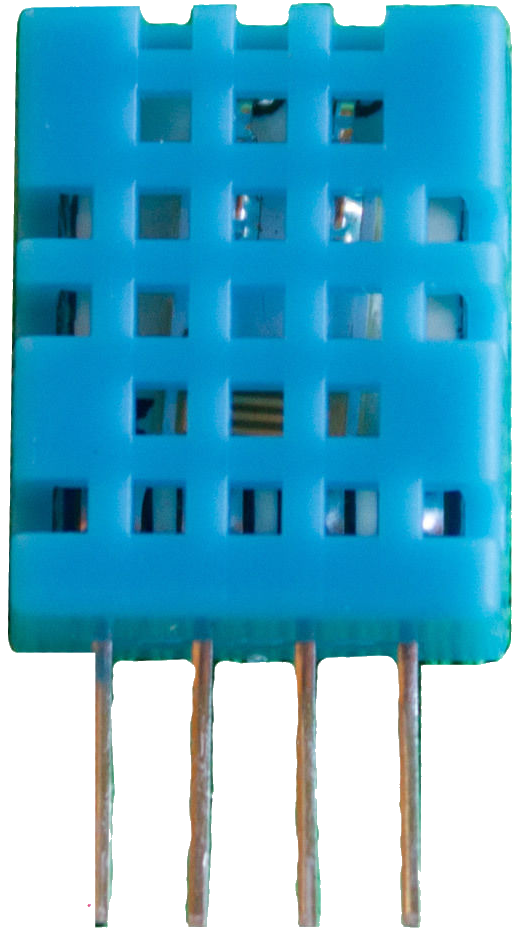
\includegraphics[align=c,height=5em]{dht11-sensor}
      \item humidity sensor
      \item magnetic hall sensor
            \hspace*{2em}
            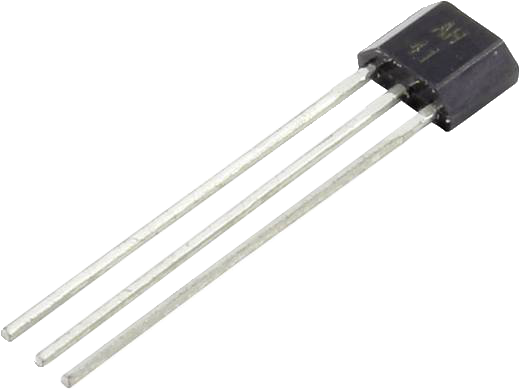
\includegraphics[align=c,height=4em]{hall-sensor}
      \item light intensity sensor
            \hspace*{2em}
            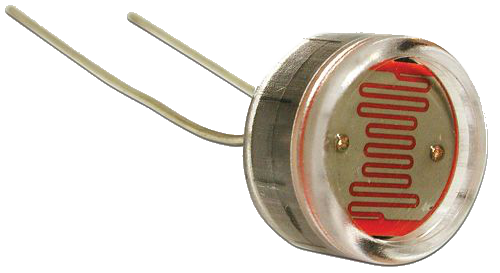
\includegraphics[align=c,height=2em]{light-sensor}
    \end{itemize}
  \end{frame}

  \begin{frame}{Raspberry Pi Application: Overview}
    \begin{itemize}
      \item written entirely in Rust
      \item cross-compiled for ARMv7
      \item collects data from 8 sensors
      \item posts sensor data as \textit{JSON} to \textit{Kafka Rest}
    \end{itemize}
  \end{frame}

  \begin{frame}{Raspberry Pi Application: Rust}
    \begin{itemize}
      \item native code, no interpreter overhead
      \item low latency for sensor measurements
      \item efficient processing of sensor data
    \end{itemize}
  \end{frame}

  \begin{frame}{Raspberry Pi Application: Sensors}
    \begin{tabularx}{\textwidth}{XC}
      \begin{itemize}
        \item built-in
          \begin{itemize}
            \item memory usage
            \item CPU load
            \item CPU temperature
          \end{itemize}
      \end{itemize}
      &
      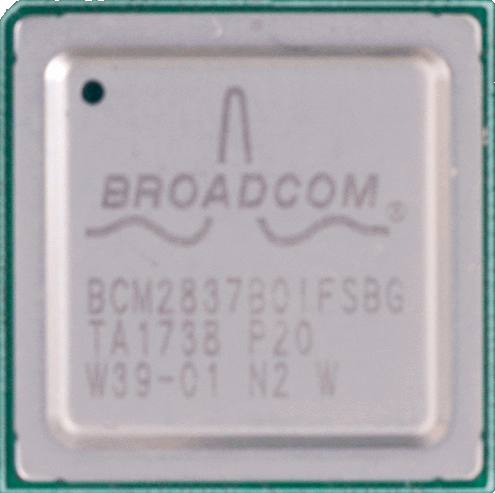
\includegraphics[valign=t,width=5em]{rpi-cpu}
      \\
      \begin{itemize}
        \item ADS1115 with photoresistor
          \begin{itemize}
            \item luminosity
          \end{itemize}
      \end{itemize}
      &
      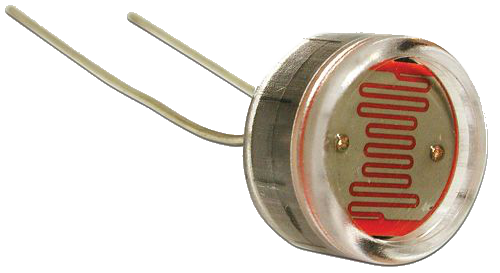
\includegraphics[valign=t,width=5em]{light-sensor}
    \end{tabularx}
  \end{frame}

  \begin{frame}{Raspberry Pi Application: Sensors}
    \begin{tabularx}{\textwidth}{XC}
      \begin{itemize}
        \item BMP180
          \begin{itemize}
            \item air pressure
            \item air temperature
          \end{itemize}
      \end{itemize}
      &
      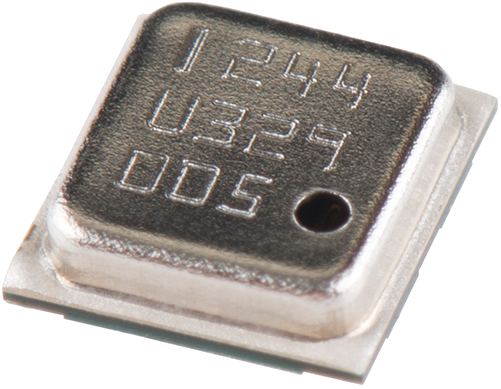
\includegraphics[valign=t,width=5em]{barometric-sensor}
      \\
      \begin{itemize}
        \item AM2320
          \begin{itemize}
            \item air humidity
            \item air temperature
          \end{itemize}
      \end{itemize}
      &
      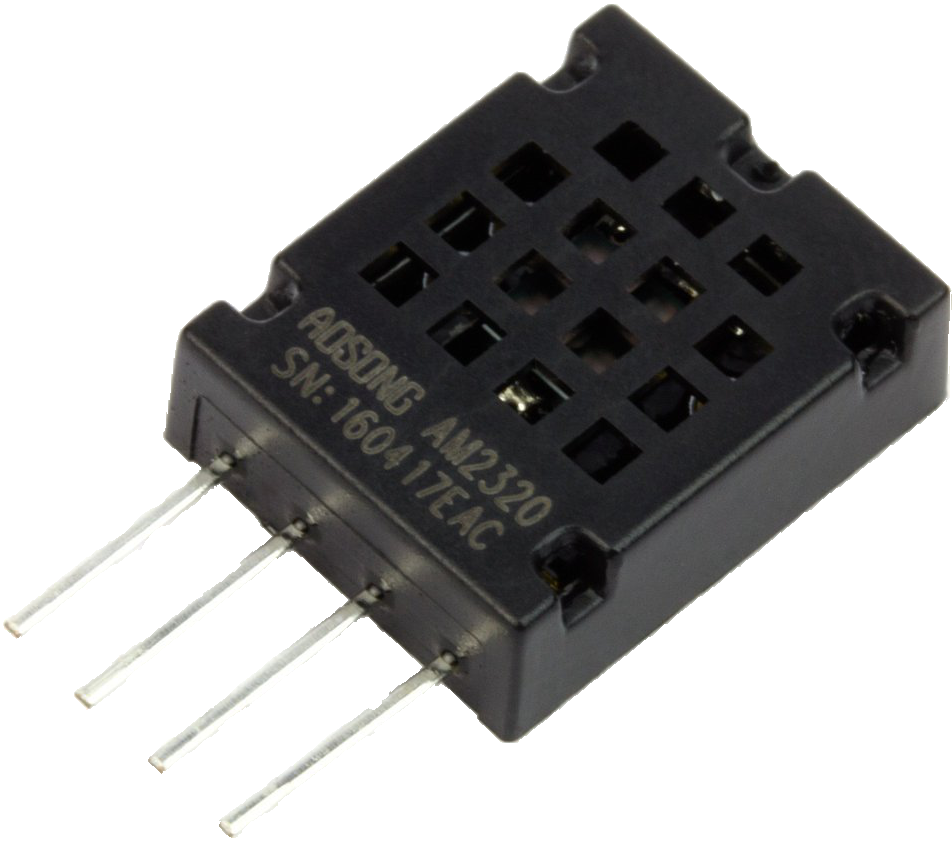
\includegraphics[valign=t,width=5em]{am2320}
    \end{tabularx}
  \end{frame}

  \begin{frame}{Background - Docker}
    
\includegraphics[height=5em]{docker-logo}

    \vspace*{1.5em}

    \begin{itemize}
      \item software packaged into containers
      \item Docker containers are standardised
      \item lightweight compared to Virtual Machines
    \end{itemize}
  \end{frame}

  \begin{frame}{Background - Docker}
    \vfill
    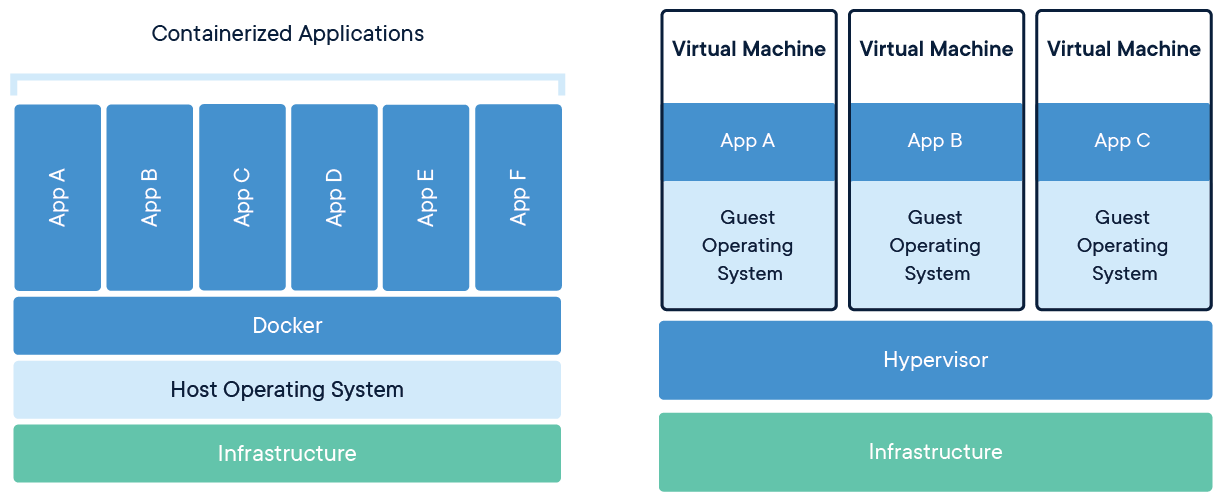
\includegraphics[width=\textwidth]{docker-containerized-and-vm}
  \end{frame}

  \begin{frame}{Background - Rust}
    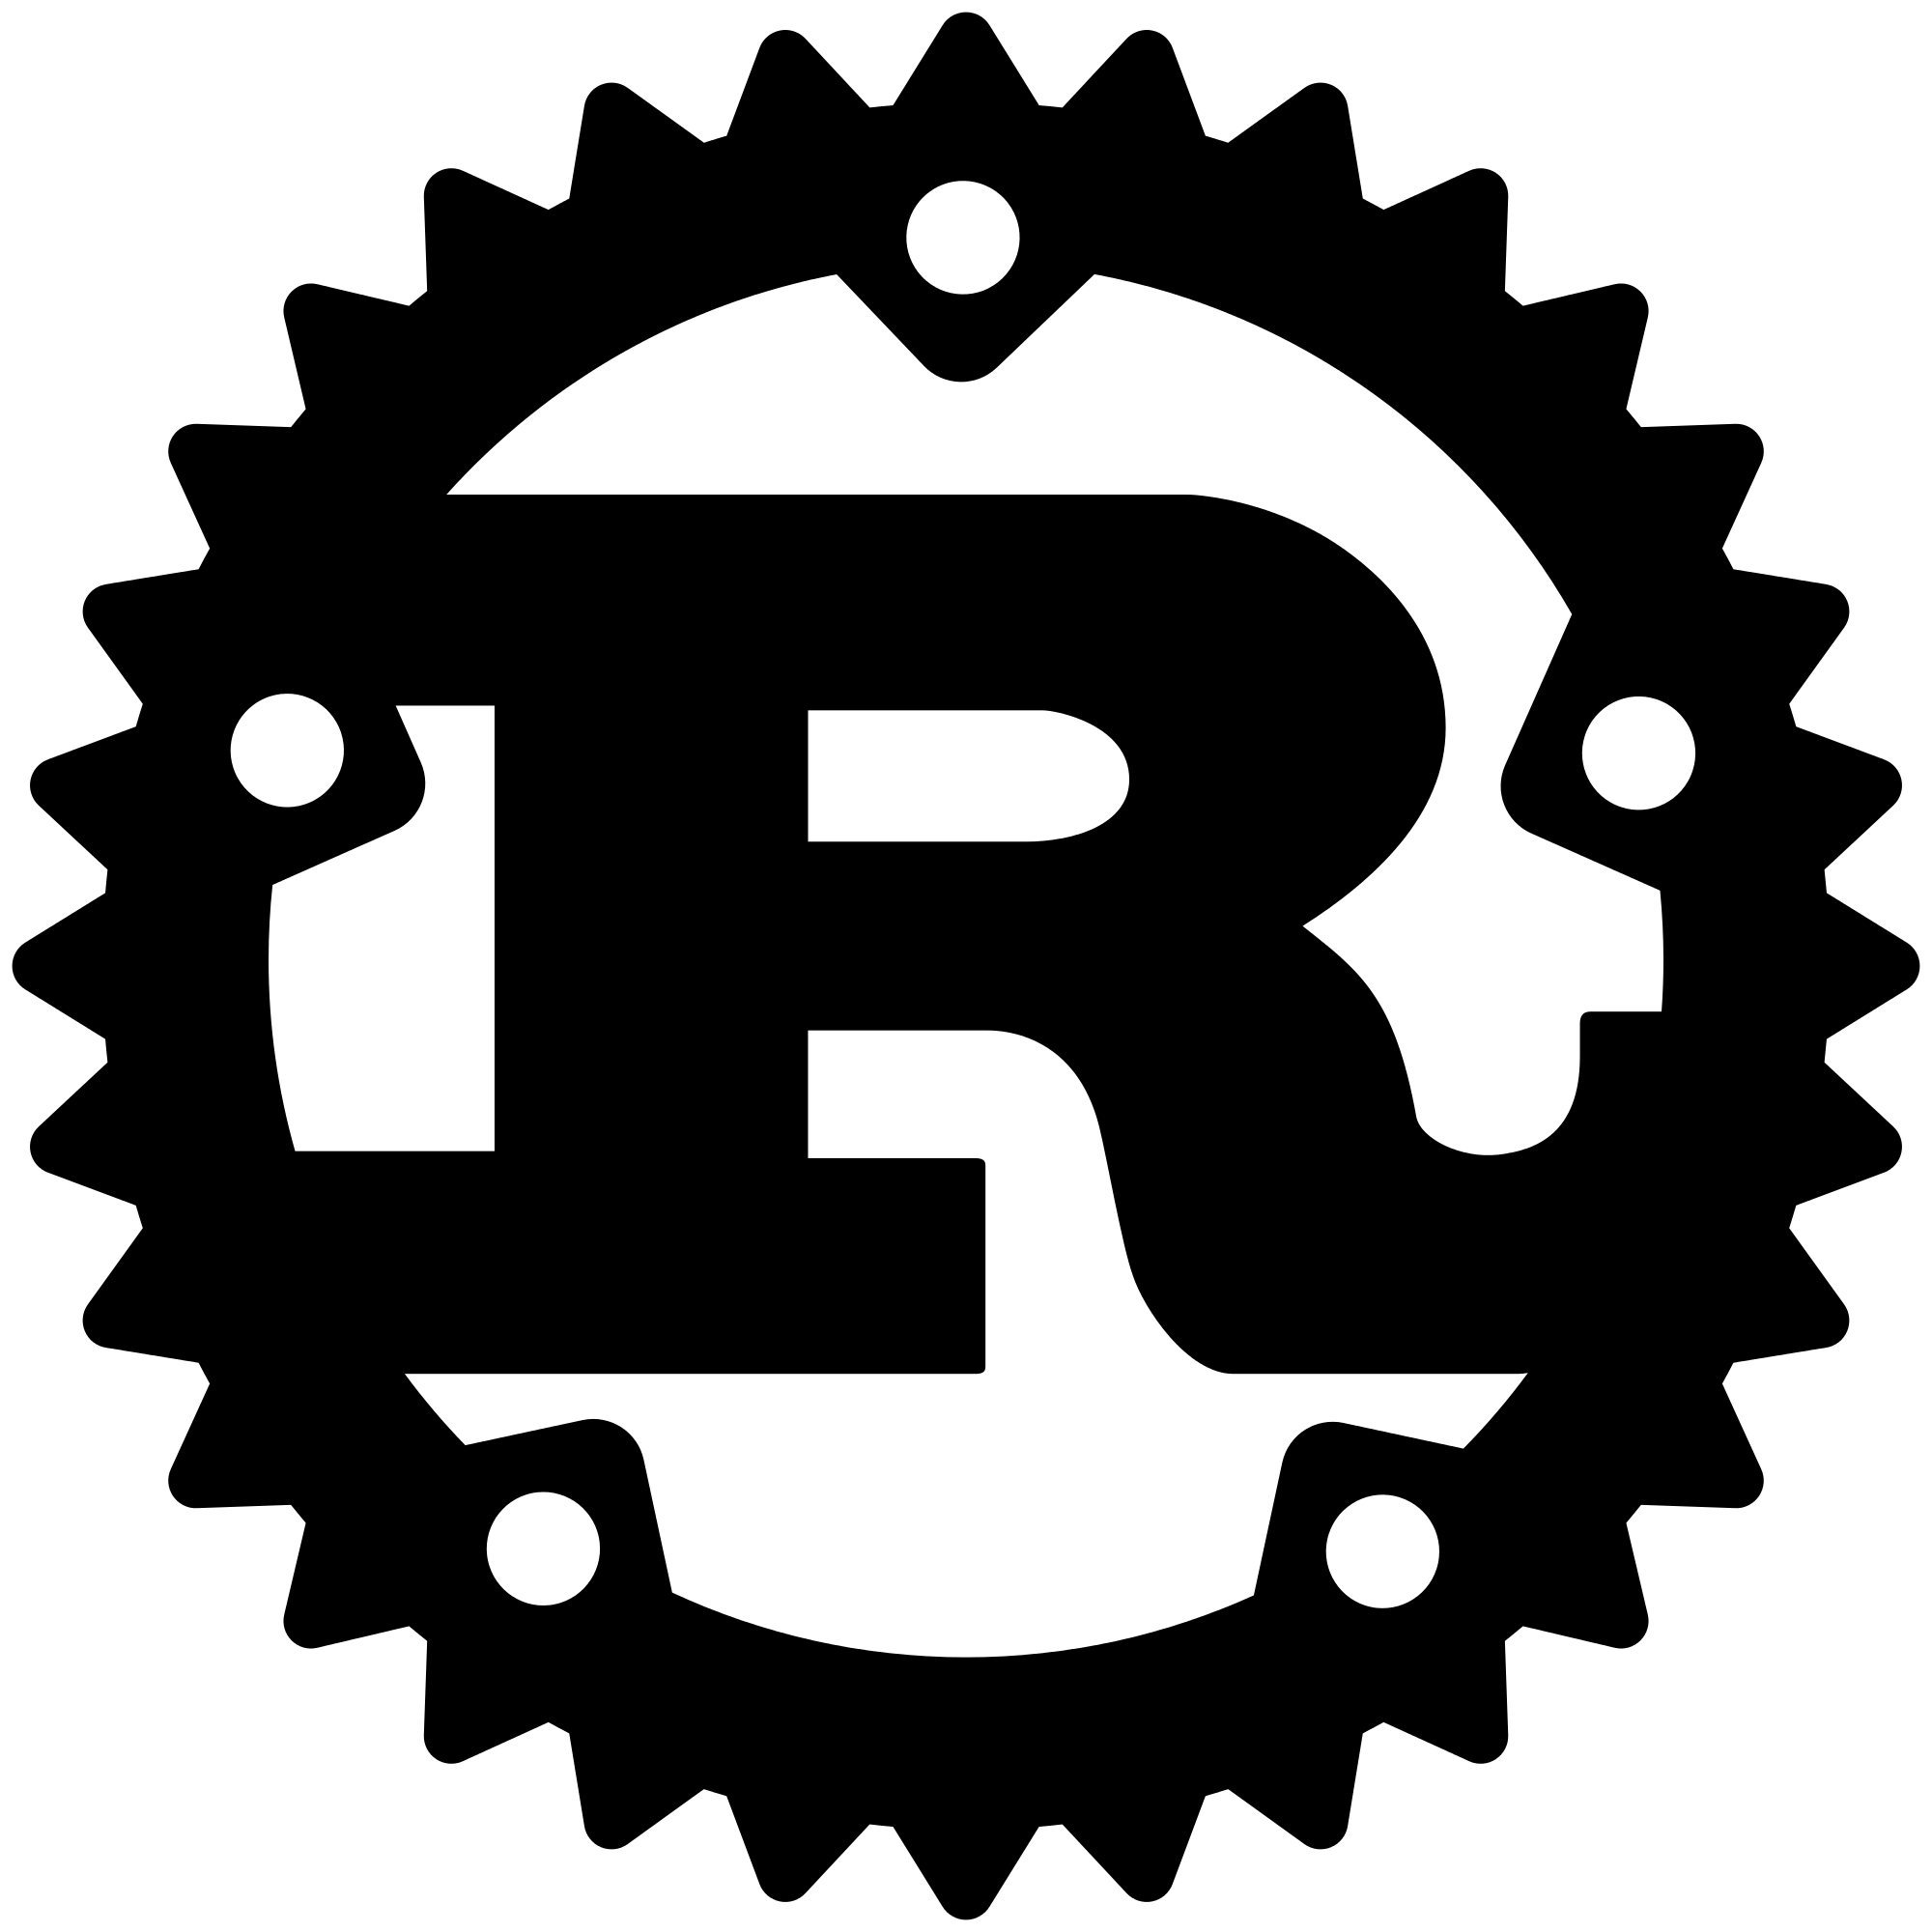
\includegraphics[height=6em]{rust-logo}

    \vspace*{1.5em}

    \begin{itemize}
      \item safe and race-condition free
      \item concurrent
      \item performant
    \end{itemize}
  \end{frame}

  \begin{frame}{Background - OpenFaaS}
    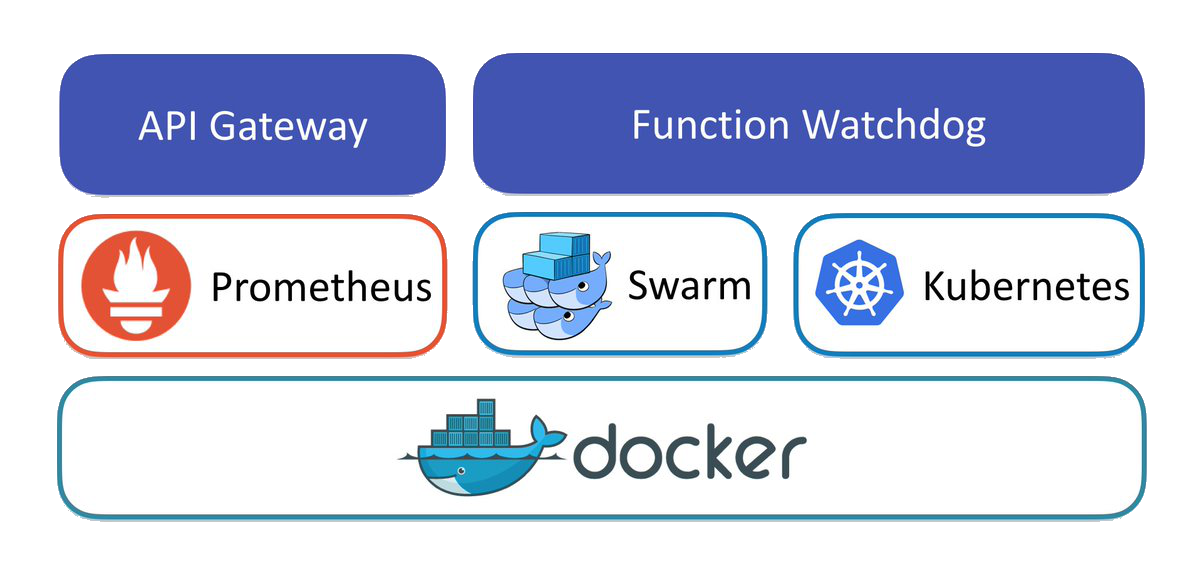
\includegraphics[width=\textwidth]{openfaas-stack}
  \end{frame}

  \begin{frame}{Background - Kafka / Zookeeper}
    
\includegraphics[height=6em]{kafka-logo}

    \vspace*{1.5em}

    \begin{itemize}
      \item devices post data to broker
      \item triggers serverless functions
    \end{itemize}
  \end{frame}

  \begin{frame}{Background - MongoDB}
    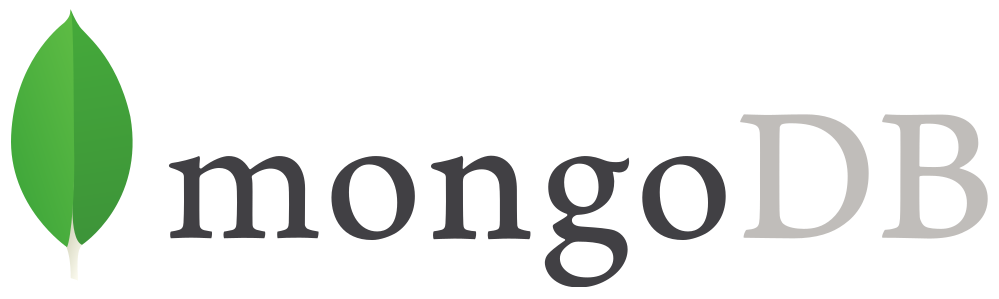
\includegraphics[height=5em]{mongodb-logo}

    \vspace*{1.5em}

    \begin{itemize}
      \item persistence layer for sensor data
      \item versatile due to its JavaScript origin
      \item JSON-like documents
    \end{itemize}
  \end{frame}

  \begin{frame}{Background - Flutter}
    
\includegraphics[height=4.5em]{flutter-logo}

    \vspace*{2em}

    \begin{itemize}
      \item cross platform UI framework from Google
      \item Dart
      \item compiles to platform native code
    \end{itemize}
  \end{frame}

  \begin{frame}{Background - MarkoJS}
    
\includegraphics[height=6em]{marko-logo}

    \vspace*{2em}

    \begin{itemize}
      \item Open Source client-side web framework from ebay
      \item similar to React
      \item support for concise syntax
    \end{itemize}
  \end{frame}

  \begin{frame}{Schedule}
    \begin{itemize}
      \item March
        \begin{itemize}
          \item setup serverless stack
          \item start mobile application
        \end{itemize}
      \item April
        \begin{itemize}
          \item finish mobile application
          \item start Raspberry Pi application
          \item start web application
        \end{itemize}
      \item May
        \begin{itemize}
          \item finish Raspberry Pi application
          \item finish web application
          \item start written part
        \end{itemize}
      \item June
        \begin{itemize}
          \item finalize bachelor’s thesis
        \end{itemize}
    \end{itemize}
  \end{frame}
\end{document}
